\chapter{}
9不会, 15答案已经给出来了
\begin{ex}
    \rmk{1} this problem reinterprets a nonrandomized test as a randomized one. 

    Given a family of probability measures 
    \(\mathcal{P}\), consider the \(\phi_{1}(\mathbf{x}):=1_{R}(\mathbf{x}), R \in \mathcal{B}\left(\mathbb{R}^{n}\right)\), called ``test 1". Now consider the following procedure (called ``test 2" ): observe \(\mathbf{x}\), and
    \[\left\{\begin{array}{l}\text { if } \mathbf{x} \in R, \text { flip an independent coin } Y \sim B(1,1) \text { and reject } H_{0} \text { if and only if } Y=1 \\ \text { if } \mathbf{x} \in R^{c}, \text { flip an independent coin } Y \sim B(1,0) \text { and reject } H_{0} \text { if and only if } Y=1\end{array}\right.\]
    Conclude that the tests 1 and 2 are equal \(\mathcal{P}\)-a.s. 
\end{ex}

\begin{solution}
    For nonrandomized test (tets 1), 
    \[
        \phi(x)=\left\{\begin{matrix}
            1 & \text{if } x \in R \\
            0 & \text{if } x \in R^{c}
        \end{matrix}\right.
    \]
    And for tets 2, 
    \[
        \left\{\begin{matrix}
            x\in R, \quad\text{reject } H_0 \text{ with probability } 1; \\
            x\in R^C, \quad\text{reject } H_0 \text{ with probability } 0. 
        \end{matrix}\right. 
    \]
    Apparently, they are equivalent. 
\end{solution}

\begin{ex}
    \rmk{2} in this problem, we calculate the size of a randomized test. 

    Assume that we want to decide between the following two distributions for a random variable \(X\) :
    \[
        H_{0}: \mathbb{P}_{0}(X=x)=\left\{\begin{array}{ll}
        0.05, & \text { if } x=2 ; \\
        0.10, & \text { if } x=1 ; \\
        0.85, & \text { if } x=0 .
        \end{array} \quad H_{1}: \mathbb{P}_{1}(X=x)= \begin{cases}0.40, & \text { if } x=2 \\
        0.50, & \text { if } x=1 \\
        0.10, & \text { if } x=0\end{cases}\right.
    \]
    Consider the (randomized) test \((n=1)\)
    \[
        \phi(x)=\left\{\begin{array}{cl}
        1, & \text { if } x=2 \\
        0.5, & \text { if } x=1 \\
        0, & \text { if } x=0
        \end{array}\right.
    \]
    This means that, once we observe \(x\), we flip an independent coin \(Y \sim B(1, \phi(x))\) and reject \(H_{0}\) if and only if \(Y=1\). Prove that \(\phi\) is a size \(0.10\) test, i.e.,
    \[
        \mathbb{E}_{0} \phi(X)=0.10
    \]
    (note that \(H_{1}\) plays no role). 
\end{ex}

\begin{solution}
    \begin{align*}
        E_0\phi(X)&=\sum \phi(X) P_0(X=x)\\
        &=0.05+0.05+0\\
        &=0.10
    \end{align*}
\end{solution}

\begin{ex}
    Let \(X_{1}, \ldots, X_{n} \stackrel{\text { i.i.d. }}{\sim} \mathcal{N}\left(\mu, \sigma_{0}^{2}\right)\), where \(\sigma_{0}^{2}\) is known. Find the MP level \(\alpha\) test for
    \[
        H_{0}: \mu=\mu_{0} \quad \text { vs } \quad H_{1}: \mu=\mu_{1}
    \]
    when \(\mu_{1}<\mu_{0}\). 
\end{ex}

\begin{solution}
    $\bar{X}$ is UMVU for $\mu$, $\bar{X}\sim \mathcal{N}(\mu, \sigma_0^2/n)$. 
    \[
        \begin{aligned}
            \frac{p_1(\bar{X})}{p_0\bar{X})}&=\exp\left(-\frac{n}{2\sigma_0^2}\left((\bar{X}-\mu_1)^2-(\bar{X}-\mu_0)^2\right)\right)\\
            &=\exp\left(-\frac{n}{2\sigma_0^2}(2\bar{X}-\mu_0-\mu_1)(\mu_0-\mu_1)\right). 
        \end{aligned}
    \]
    This ratio is decreasing  for $\bar{X}$. So, $\frac{p_1(x)}{p_0(x)}>c$ equals to $\bar{X}<c'$. 
    \[
        P_0(\bar{X}<c')=\alpha. 
    \]
    \[
        P_0\left(\frac{\bar{X}-\mu}{\sigma/\sqrt{n}}<\frac{c'-\mu}{\sigma/\sqrt{n}}\right)=\alpha. 
    \]
    \[
        c'=\frac{\sigma}{\sqrt{n}}z_\alpha+\mu_0. 
    \]
    Finally, the MP test is: Reject $H_0$ if $\bar{X}<c'$. 
\end{solution}

\begin{ex}
    A lot of items contains the proportion \(p\) of defectives. The lot is large enough so that it is reasonable to assume individual items selected at random without replacement are independent Bernoulli trials with parameter \(p\). Suppose \(n\) items are selected at random. We want to test
    \[
        H_{0}: p=0.1 \quad \text { vs } \quad H_{1}: p=0.2
    \]
    Considering only nonrandomized tests, prove that the MP level \(\alpha\) test rejects in the region
    \begin{equation}
        \label{eq:8.4}
        \left\{\mathbf{x}: \sum_{i=1}^{n} x_{i}>c(\alpha)\right\}. 
    \end{equation}
    for appropriate values of \(\alpha\) (n.b.: there are only finitely many values of \(\alpha\) such that the nonrandomized test (\ref{eq:8.4}) is \(\mathrm{MP})\). Indicate how one calculates \(c\) as a function of \(\alpha\). 
\end{ex}

\begin{solution}
    Because $x_i\sim Ber(p)$, then $X'=\sum x_i\sim B(n,p)$. 
    \begin{align*}
        \frac{p_1(X')}{p_0(X')}&=2^x(8/9)^{n-x}. 
    \end{align*}
    This ratio is increasing for $X'$. So, $\frac{p_1(x')}{p_0(x')}>c$ equals to $X'>c'$. Then
    \[
        P_0(X'>c')=\alpha; 
    \]
    \[
        \sum_{i=c'+1}^{n} \binom{n}{i}p^i(1-p)^{n-i}=\alpha.
    \]
    From this equation, we can calculate \(c'\) as a function of \(\alpha\). 
\end{solution}

\begin{ex}
    Let \(X_{1}, \ldots, X_{n} \stackrel{\text { i.i.d. }}{\sim} \exp (\lambda)\). For \(\lambda_{0}>0\), we want to test
    \[
        H_{0}: \lambda \leq \lambda_{0} \quad \text { vs } \quad H_{1}: \lambda>\lambda_{0} .
    \]
    Find the UMP level \(\alpha\) test. 
\end{ex}

\begin{solution}
    \[
        f(x, \lambda)=\lambda^n\exp\left(-\lambda\sum x_i\right), 
    \]
    For $\lambda'>\lambda$, 
    \[
        \frac{\lambda'^n\exp\left(-\lambda'\sum x_i\right)}{\lambda^n\exp\left(-\lambda\sum x_i\right)}=\left(\frac{\lambda'}{\lambda}\right)^n\exp\left((\lambda-\lambda')\sum x_i\right). 
    \]
    It is decreasing for $T(X)=\sum x_i$. So, this $H_0$ has UMP level $\alpha$ test: 
    \[
        \phi(X)=\left\{\begin{matrix}
            1, & \text{if } T(X)<c\\
            0, & \text{if } T(X)>c
        \end{matrix}\right.
    \]
    \[
        E_{\lambda_0}(\phi(X))=\alpha. 
    \]
    And $M_x(t)=(1-t/\lambda)^{-1}$, $M_{T(X)}(t)=(1-t/\lambda)^{-n}$. $M_{2n\lambda_0T(X)}(t)=(1-2t)^{-2n/2}$. So, 
    \[
        2n\lambda_0T(X)\sim \chi^2(2n). 
    \]
    \[
        P(2n\lambda_0T(X)<2n\lambda_0c)=\alpha\Rightarrow c=\chi^2_{\alpha}(2n)/(2n\lambda_0). 
    \]
\end{solution}


\begin{ex}
    Let \(X_{1}, \ldots, X_{n} \stackrel{\text { i.i.d. }}{\sim} \mathcal{N}\left(\mu, \sigma_{0}^{2}\right)\), where \(\sigma_{0}^{2}\) is known. Prove that the family of distributions has a MLR with respect to \(\bar{X}\). 
\end{ex}

\begin{solution}
    \[
        f(x, \mu)=\left(\frac{1}{\sqrt{2\pi}\sigma_0}\right)^n\exp\left(-\frac{1}{2\sigma_{0}^{2}}\sum\left(x_i-\mu\right)^2\right)
    \]
    For $\mu'>\mu$, 
    \[\begin{aligned}
        \frac{f(x,\mu')}{f(x,\mu)}&=\exp\left(\frac{1}{2\sigma_0^2}(\mu'-\mu)\left(-2\sum x_i+n(\mu'+\mu)\right)\right)\\
        &=\exp\left(\frac{1}{2\sigma_0^2}(\mu'-\mu)\left(-2n\bar{X}+n(\mu'+\mu)\right)\right)
    \end{aligned}
    \]
    For $T(X)=\bar{X}$, the ratio is nonincreasing. So, it has a MLR. 
\end{solution}

\begin{ex}
    Let \(\mathcal{P}\) be a one-parameter canonical exponential family generated by \(T(x)\) and \(\mathcal{E}=\operatorname{int} \mathcal{E} \neq \emptyset\). Show that \(\mathcal{P}\) has a MLR with respect to \(T(x)\). 
\end{ex}

\begin{solution}
    \[
        f(x, \eta)=h(x)\exp\left(\eta T(x)-A(\eta)\right), 
    \]
    For $\eta'>\eta$, 
    \[
        \begin{aligned}
            \frac{f(x,\eta')}{f(x,\eta)}&=\exp\left((\eta'-\eta)T(x)+A(\eta)-A(\eta')\right)
        \end{aligned}
    \]
    It is monotone increasing for $T(X)$, hence, it has a MLR. 
\end{solution}

\begin{ex}
    Suppose that the assumptions of the Neyman-Pearson lemma hold for hypotheses of the form
    \[
        H_{0}: \theta=\theta_{0} \quad \text { vs } \quad H_{1}: \theta=\theta_{1} .
    \]
    For a given \(\alpha\), let \(\pi\left(\theta_{1}\right)\) be the power of the MP test. We would like to show that \(\alpha<\pi\left(\theta_{1}\right)\). 
    \begin{enumerate}[(a)]
        \item Define the test \(\psi(\mathbf{x}) \equiv \alpha\), i.e., irrespective of \(\mathbf{x}\), it rejects \(H_{0}\) with probability \(\alpha\) (remark: this is a randomized test). Conclude that \(\alpha \leq \pi\left(\theta_{1}\right)\). 
        \item Assume that \(\alpha=\pi\left(\theta_{1}\right)\). Conclude that \(\psi(\mathbf{x})\) is \(\mathrm{MP}\), and arrive at a contradiction with one of the assumptions of the Neyman-Pearson lemma. 
    \end{enumerate}
\end{ex}

\begin{solution}
    \begin{enumerate}[(a)]
        \item \[\alpha=E_0(\psi(x))< E_1(\psi(x))\leqslant\pi(\theta_1). \]
        and $\pi(\theta)=\alpha$. So, $\alpha\leqslant\pi(\theta)$. 
        \item If $\alpha=\pi(\theta_1)$, and because $\alpha=\sup_{\theta\in\Theta_0}\pi(\theta)$, which means no other test has large power than $\psi$, i.e., $\psi$ is MP. Then, $E_0(\psi)=E_1(\psi)\Rightarrow p_0=p_1$. Here we get the contradiction. 
    \end{enumerate}
\end{solution}

\begin{ex}
    (in this problem, we show the Karlin-Rubin theorem)

    Suppose that the family \(\mathcal{P}=\) \(\{f(\mathbf{x} \mid \theta)\}_{\theta \in \Theta}\) has MLR with respect to \(T(\mathbf{x})\), and we are willing to test the hypothesis
    \[
        H_{0}: \theta \leq \theta_{0} \quad \text { vs } \quad H_{1}: \theta>\theta_{0}. 
    \]
    \begin{enumerate}[(a)]
        \item Consider first the simple hypothesis
        \[
        H_{0}: \theta=\theta_{0} \quad \text { vs } \quad H_{1}: \theta=\theta_{1}>\theta_{0}
        \]
        Show that the test that rejects for large values of \(T(\mathbf{x})\) is MP. 
        \item For a fixed, pre-chosen \(\alpha\), show that there are \(c\) and \(\gamma\) such that
        \[
        \phi(\mathbf{x})=\left\{\begin{array}{ll}
        1, & \text { if } T(\mathbf{x})>c \\
        0, & \text { if } T(\mathbf{x})<c ; \\
        \gamma, & \text { if } T(\mathbf{x})=c
        \end{array} \quad \mathbb{E}_{\theta_{0}} \phi(\mathbf{X})=\alpha\right.
        \]
        (hint: use the argument in the existence part of the Neyman-Pearson lemma).
        \item Conclude that the test obtained in (b) is also MP for testing \(\theta^{\prime}\) against \(\theta^{\prime \prime}, \theta^{\prime}<\theta^{\prime \prime}\), at level \(\alpha^{\prime}=\pi\left(\theta^{\prime}\right)\). 
        \item Show that the power function
        \[
            \pi\left(\theta^{\prime}\right)=\mathbb{E}_{\theta^{\prime}} \phi(\mathbf{X})
        \]
        is strictly increasing (hint: use the previous problem). 
        \item Let \(\psi(\mathbf{X})\) be any test, and consider the condition
        \item 
        \begin{equation}
            \label{eq:8.9.e.1}
            \mathbb{E}_{\theta} \psi(\mathbf{X}) \leq \alpha, \quad \theta \leq \theta_{0}. 
        \end{equation}
        Conclude that \(\psi(\mathbf{X})\) also satisfies
        \begin{equation}
            \label{eq:8.9.e.2}
            \mathbb{E}_{\theta_{0}} \psi(\mathbf{X}) \leq \alpha. 
        \end{equation}
        \item Conclude that \(\phi(\mathbf{X})\) satisfies the condition (\ref{eq:8.9.e.1}) and that it is MP (with respect to \(\theta_{1}\) ) in the broader class of tests that satisfy (\ref{eq:8.9.e.2}). 
        \item Conclude that \(\phi(\mathbf{X})\) is UMP against \(H_{1}\). 
        
        (hint: use (f) and the fact that \(\phi(\mathbf{X})\) is independent of the particular \(\theta_{1}\) chosen). 
    \end{enumerate}
\end{ex}

\begin{solution}
    \begin{enumerate}[(a)]
        \item 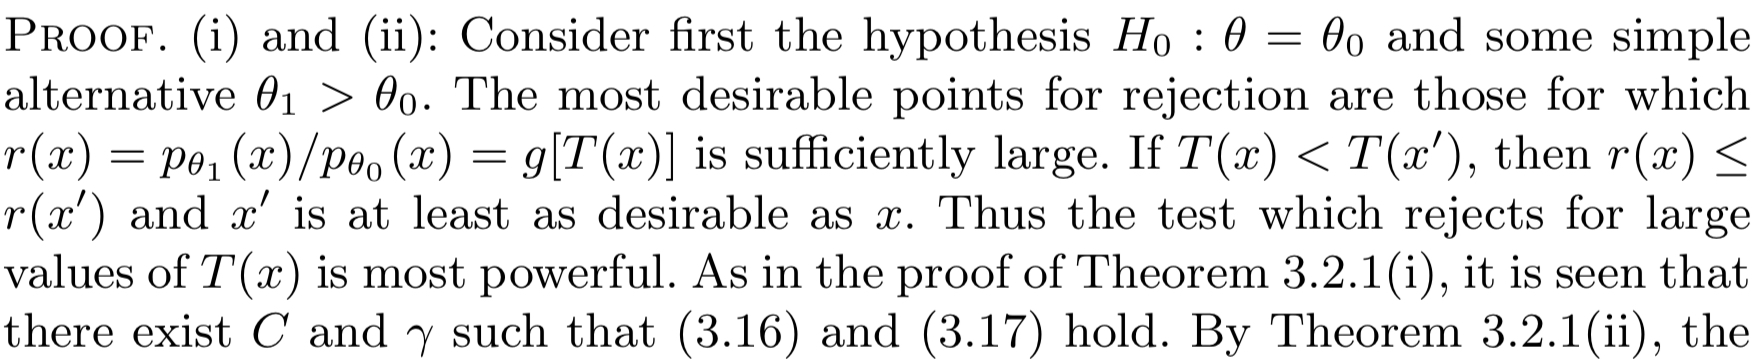
\includegraphics[width=.9\textwidth]{Proof 1.jpeg}
        \item 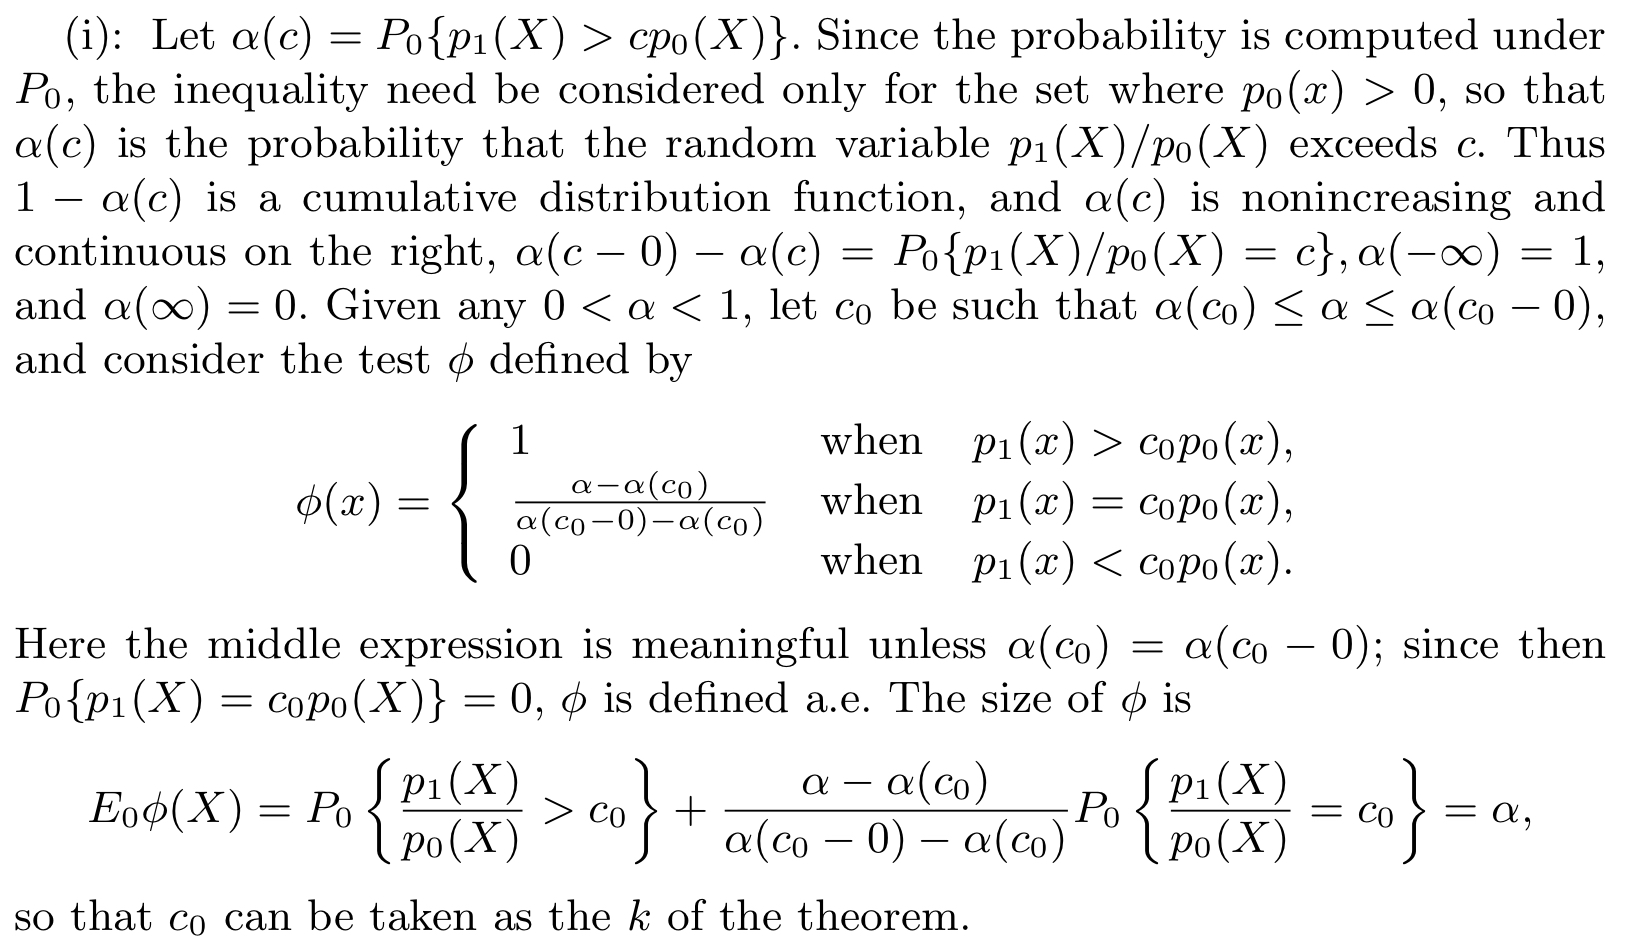
\includegraphics[width=.9\textwidth]{Proof 2.png}
        \item From NP-lemma existence, it is also MP. 
        \item Since $\pi(\theta)$ is nondecreasing 
    \end{enumerate}
\end{solution}


\begin{ex}
    Let \(X_{1}, \ldots, X_{n} \stackrel{\text { i.i.d. }}{\sim} \mathcal{N}\left(\mu, \sigma^{2}\right)\), where both parameters are unknown. Prove that the GLR tests have the form
    \[
        \begin{array}{ccc}
        \hline H_{0} & H_{1} & R \\
        \hline \mu \leq \mu_{0} & \mu>\mu_{0} & \bar{x}>\mu_{0}+\frac{s}{\sqrt{n}} t_{\alpha} \\
        \mu \geq \mu_{0} & \mu<\mu_{0} & \bar{x}<\mu_{0}-\frac{s}{\sqrt{n}} t_{\alpha} \\
        \mu=\mu_{0} & \mu \neq \mu_{0} & \left|\frac{\bar{x}-\mu_{0}}{s / \sqrt{n}}\right|>t_{\alpha / 2} \\
        \hline
        \end{array}
    \]
\end{ex}

\begin{solution}
    \begin{itemize}
        \item \[
            \mathcal{L}=\left(\frac{1}{\sqrt{2\pi}\sigma}\right)^n \exp\left(-\frac{1}{2\sigma^2}\sum\left(x_i-\mu\right)^2\right). 
        \]
        If there is no any restriction for $\mu$, then the MLE for $\mu$ is $\bar{X}$, and the MLE for $\sigma^2$ is $\frac{\sum(x_i-\bar{x})^2}{n}$. However, with $\mu<\mu_0$, the MLE for $\mu$ is $\bar{x}$, when $\bar{x}\leqslant\mu_0$; but when $\bar{x}>\mu_0$, the MLE for $\mu$ is $\mu_0$. Same with the MLE for $\sigma^2$. i.e., when $\bar{x}\leqslant\mu_0$, MLE is $\frac{\sum(x_i-\bar{x})^2}{n}$, and when $\bar{x}>\mu_0$, MLE is $\frac{\sum(x_i-\mu_0)^2}{n}$. 

        Noticing that when $\bar{x}\leqslant\mu_0$, $\mathcal{L}_0=\mathcal{L}_1\Rightarrow\frac{\mathcal{L}_0}{\mathcal{L}_1}=1$. And in this case, we always accept $H_0$. When $\bar{x}>\mu_0$, the reject region is: 
        \begin{align*}
            \frac{\mathcal{L}_0}{\mathcal{L}_1}&=\left(\frac{\sum(x_i-\bar{x})^2}{\sum(x_i-\mu_0)^2}\right)^{n/2}<c\\
            &\Rightarrow  \frac{\sum(x_i-\mu_0)^2}{\sum(x_i-\bar{x})^2}>c_1\\
            &\Rightarrow  \frac{\sum(x_i-\bar{x})^2+n(\bar{x}-\mu_0)^2}{\sum(x_i-\bar{x})^2}>c_2\\
            &\Rightarrow  \frac{n(\bar{x}-\mu_0)^2}{\sum(x_i-\bar{x})^2}>c_3\\
            &\Rightarrow  \sqrt{\frac{(\bar{x}-\mu_0)^2}{\sum(x_i-\bar{x})^2/n}}>c_4\\
            &\Rightarrow  \frac{\bar{x}-\mu_0}{S/\sqrt{n}}>c_5. 
        \end{align*}
        where $\frac{\bar{x}-\mu_0}{S/\sqrt{n}}\sim t(n-1)$. 
        So, the Reject Region is:
        \[
            \frac{\bar{x}-\mu_0}{S/\sqrt{n}}>t_{1-\alpha}(n-1)\Rightarrow\bar{x}>\mu_0+\frac{S}{\sqrt{n}} t_{1-\alpha}(n-1). 
        \]
        \item For $H_0: \mu\geqslant \mu_0$, we just need to reverse the inequality sign, and get the Reject Region:
        \[
            \frac{\bar{x}-\mu_0}{S/\sqrt{n}}<t_{\alpha}(n-1)\Rightarrow\bar{x}<\mu_0+\frac{S}{\sqrt{n}} t_{\alpha}(n-1). 
        \]
        \item Same, the Reject Region is: 
        \[
            \left|\frac{\bar{x}-\mu_0}{S/\sqrt{n}}\right|>t_{1-\alpha/2}(n-1). 
        \]
    \end{itemize}
\end{solution}

\begin{ex}
    Let \(X_{1}, \ldots, X_{n} \stackrel{\text { i.i.d. }}{\sim} \mathcal{N}\left(\mu, \sigma^{2}\right)\), where both parameters are unknown. Prove that the GLR tests have the form
    \begin{center}
        \begin{tabular}{ccc}
            \hline\(H_{0}\) & \(H_{1}\) & \(R\) \\
            \hline\(\sigma^{2} \leq \sigma_{0}^{2}\) & \(\sigma^{2}>\sigma_{0}^{2}\) & \(\frac{(n-1) s^{2}}{\sigma_{0}^{2}}>\chi_{n-1}^{2}(\alpha)\) \\
            \(\sigma^{2} \geq \sigma_{0}^{2}\) & \(\sigma^{2}<\sigma_{0}^{2}\) & \(\frac{(n-1) s^{2}}{\sigma_{0}^{2}}<\chi_{n-1}^{2}(1-\alpha)\) \\
            \(\sigma^{2}=\sigma_{0}^{2}\) & \(\sigma^{2} \neq \sigma_{0}^{2}\) & \(\left\{\frac{(n-1) s^{2}}{\sigma_{0}^{2}}<\chi_{n-1}^{2}(1-\alpha / 2)\right\} \cup\left\{\frac{(n-1) s^{2}}{\sigma_{0}^{2}}>\chi_{n-1}^{2}(\alpha / 2)\right\}\) \\
            \hline
        \end{tabular}
    \end{center}
\end{ex}

\begin{solution}
    \begin{itemize}
        \item \[
            \mathcal{L}=\left(\frac{1}{\sqrt{2\pi}\sigma}\right)^n \exp\left(-\frac{1}{2\sigma^2}\sum\left(x_i-\mu\right)^2\right). 
        \]
        When $\frac{\sum(x_i-\bar{x})^2}{n}>\sigma_0^2$, 
        \begin{align*}
            \frac{\mathcal{L}_0}{\mathcal{L}_1}&=\left(\frac{\sigma^2}{\sigma_0^2}\right)^{n/2}\exp\left(-\frac{n}{2}\frac{\sigma^2}{\sigma_0^2}\right). 
        \end{align*}
        This ratio first increase before $\sigma^2/\sigma_0^2=1$, then decrease. So, the Reject Region is: 
        \[
            \sigma^2/\sigma_0^2<c_1<1, \text{ and } \sigma^2/\sigma_0^2>c_2>1.
        \]
        We accept $H_0$ when $\sigma^2/\sigma_0^2<1$, 
        \[
            \begin{aligned}
                &\sigma^2/\sigma_0^2>c_2\\
                \Rightarrow &\frac{\sum(x_i-\bar{x})^2}{n\sigma_0^2}>c_2\\
                \Rightarrow &\frac{(n-1)s^2}{\sigma_0^2}>c_3. 
            \end{aligned}
        \]
        And $\frac{(n-1)s^2}{\sigma_0^2}\sim\chi^2(n-1)$. So, the Reject Region is:
        \[
            \frac{(n-1)s^2}{\sigma_0^2}>\chi^2_{1-\alpha}(n-1). 
        \]
        \item Same, the Reject Region is:
        \[
            \frac{(n-1)s^2}{\sigma_0^2}<\chi^2_{\alpha}(n-1). 
        \]
        \item The Reject Region is:
        \[
            \left\{\frac{(n-1)s^2}{\sigma_0^2}<\chi^2_{\alpha/2}(n-1)\right\}\bigcup\left\{\frac{(n-1)s^2}{\sigma_0^2}>\chi^2_{1-\alpha/2}(n-1)\right\}
        \]
    \end{itemize}
\end{solution}

\begin{ex}
    Suppose we have two independent samples: \(X_{1}, \ldots, X_{n} \stackrel{\text { i.i.d. }}{\sim} \exp \left(\lambda_{1}\right), Y_{1}, \ldots, Y_{m} \stackrel{\text { i.i.d. }}{\sim} \exp \left(\lambda_{2}\right)\). 
    \begin{enumerate}[(a)]
        \item Find the GLR test for the hypotheses
        \[
        H_{0}: \lambda_{1}=\lambda_{2} \quad \text { vs } \quad H_{1}: \lambda_{1} \neq \lambda_{2}. 
        \]
        (remark: note that the definition of GLR tests does encompass this two-sample case). 
        \item Show that the test in part (a) can be based on the statistic
        \[
        T(\mathbf{X}, \mathbf{Y})=\frac{\sum_{i=1}^{n} X_{i}}{\sum_{i=1}^{n} X_{i}+\sum_{j=1}^{m} Y_{j}}. 
        \]
        \item Find the distribution of \(T(\mathbf{X}, \mathbf{Y})\) when \(H_{0}\) is true. 
    \end{enumerate}
    (hint: for (b), express \(\Lambda(\mathbf{x}, \mathbf{y})\) as a function of \(T(\mathbf{x}, \mathbf{y})\), and note that \(\Lambda(\mathbf{x}, \mathbf{y})\) is unimodal with respect to \(T(\mathbf{x}, \mathbf{y})\). Now conclude that \(\Lambda(\mathbf{x}, \mathbf{y})\) is small if and only if \(T(\mathbf{x}, \mathbf{y})\) is small or large. For (c), \(\sum_{i} X_{i}\) and \(\sum_{j} Y_{j}\) follow Gamma distributions; there is a relation between Gamma and Beta random variables).
\end{ex}

\begin{solution}
        \[
            \mathcal{L}(\lambda_1, \lambda_2)=\lambda_1^n\lambda_2^m\exp\left(-\lambda_1\sum^nX_i-\lambda_2\sum^mY_i\right), 
        \]
        $\hat{\lambda}_1=\frac{1}{\bar{X}}$, $\hat{\lambda}=\frac{n+m}{n\bar{X}+m\bar{Y}}$, 
        \[
            \frac{\mathcal{L}_0}{\mathcal{L}_1}=\frac{(n+m)^{n+m}}{n^nm^m}\frac{(n\bar{X})^n(m\bar{Y})^m}{(n\bar{X}+m\bar{Y})^{n+m}}. 
        \]
        Let $T(X)=n\bar{x}/(n\bar{x}+m\bar{y})$, 
        \[
            \begin{aligned}
                \frac{\mathcal{L}_0}{\mathcal{L}_1}<c&\Rightarrow \frac{(n+m)^{n+m}}{n^nm^m}\frac{(n\bar{X})^n(m\bar{Y})^m}{(n\bar{X}+m\bar{Y})^{n+m}}<c\\
                &\Rightarrow  T(X)^m(1-T(X))^n<c_1. 
            \end{aligned}
        \]
        this function of $T(X)$ will increase before $T(X)=m/(m+n)$, then. after $m/(m+n)$, it will decrease. So, the Reject Region is:
        \[
            T(X)<c_l, \text{ and } T(X)>c_r.
        \]
        $X\sim Exp(\lambda_1)$, $2n\lambda\bar{X}\sim \chi^2(2n)$. \[
            \frac{n\bar{x}}{n\bar{x}+m\bar{y}}=\frac{2\lambda n\bar{x}}{2\lambda n\bar{x}+2\lambda m\bar{y}}\sim\frac{\chi^2(2n)}{\chi^2(2n+2m)}=F(2n,2m+2n). 
        \]
        So, the Reject Region is:
        \[
            \left\{T(X)<F_{\alpha/2}(2n,2m+2n)\right\} \bigcup \left\{T(X)>F_{1-\alpha/2}(2n,2m+2n)\right\} 
        \]
\end{solution}

\begin{ex}
    Let \(X_{1}, \ldots, X_{n} \stackrel{\text { i.i.d. }}{\sim} \mathcal{N}\left(\mu_{1}, \sigma^{2}\right)\) and \(Y_{1}, \ldots, Y_{m} \stackrel{\text { i.i.d. }}{\sim} \mathcal{N}\left(\mu_{2}, \sigma^{2}\right)\) be two independent samples. We are interested in testing
    \[
        H_{0}: \mu_{1}=\mu_{2} \quad \text { vs } \quad H_{0}: \mu_{1} \neq \mu_{2} .
    \]
    \begin{enumerate}[(a)]
        \item Derive the GLR test. Show that it can be based on the statistic
        \[
            T(\mathbf{x}, \mathbf{y})=\frac{\bar{X}-\bar{Y}}{\sqrt{S_{p}^{2}\left(\frac{1}{n}+\frac{1}{m}\right)}}, \quad S_{p}^{2}=\frac{1}{n+m-2}\left(\sum_{i=1}^{n}\left(X_{i}-\bar{X}\right)^{2}+\sum_{j=1}^{m}\left(Y_{j}-\bar{Y}\right)^{2}\right). 
        \]
        \item Show that
        \[
            T(\mathbf{x}, \mathbf{y}) \sim t_{n+m-2} \quad \text { under } H_{0} .
        \]
    \end{enumerate}
    In other words, the GLR test is equivalent to the so-called two-sample \(t\) test (remark: the case where the variances from the two samples are potentially distinct is called the Behrens-Fisher problem, and it is surprisingly intricate). 
\end{ex}

\begin{solution}
    If $H_0$ is true: 
    $\hat{\mu}=(\sum^nx_i+\sum^my_i)/(m+n)$, $\hat{\sigma}^2=(\sum^n(x_i-\mu)^2+\sum^m(y_i-\mu)^2)/(m+n)$. 

    \noindent If $\mu_1\neq\mu_2$, then $\hat{\mu}_1=\bar{X}$, $\hat{\mu}_2=\bar{Y}$, $\hat{\sigma}^2=(\sum^n(x_i-\mu_1)^2+\sum^m(y_i-\mu_2)^2)/(m+n)$. 
    \[
        \frac{\mathcal{L}_0}{\mathcal{L}_1}=\left(1+\frac{(T(x,y))^2}{m+n-2}\right)^{(m+n)/2}. 
    \]
    这个式子没算出来, 网上找的结果. 
    \[
        \bar{X}\sim N(\mu_1, \sigma^2/n), 
        \bar{Y}\sim N(\mu_2, \sigma^2/m), \bar{X}-\bar{Y}\sim N(\mu_1-\mu_2, \sigma^2(1/n+1/m)),
    \]
    \[
        \frac{\bar{X}-\bar{Y}}{S\sqrt{\frac{1}{n}+\frac{1}{m}}}\sim t(n+m-2), \quad S^2=\frac{1}{n+m-2}\left(\sum_{i=1}^{n}\left(X_{i}-\bar{X}\right)^{2}+\sum_{j=1}^{m}\left(Y_{j}-\bar{Y}\right)^{2}\right). 
    \]
\end{solution}

\begin{ex}
    Consider the hypotheses
    \(H_{0}: f_{0}(\mathbf{x})\) is true vs \(H_{1}: f_{1}(\mathbf{x})\) is true,
    where \(f_{j}(\mathbf{x}), j=0,1\), are generalized densities with respect to some \(\sigma\)-finite measure \(G(d \mathbf{x})\) and satisfying the identifiability condition \(G\left(\left\{\mathbf{x}: f_{1}(\mathbf{x}) \neq f_{0}(\mathbf{x})\right\}\right)>0\) (cf. the NeymanPearson lemma). Assume the distribution of the likelihood ratio statistic \(\frac{f_{1}(\mathbf{X})}{f_{0}(\mathbf{X})}\) is continuous under \(H_{0}\) (i.e., the c.d.f. of \(\frac{f_{1}(\mathbf{X})}{f_{0}(\mathbf{X})}\) is continuous). Show that the rejection regions of the MP test are nested, i.e.,
    \[
        \alpha<\alpha^{\prime} \Rightarrow R_{\alpha} \subseteq R_{\alpha^{\prime}}. 
    \]
\end{ex}

\begin{solution}
    From NP-lemma, for  $\alpha<\alpha'$, there are $c$, $c'$, such that the critical region are $f_1/f_0>c$, $f_1/f_0>c'$ respectively. And 
    \[
        \alpha=P_0(f_1/f_0>c)<P_0(f_1/f_0>c')=\alpha'. 
    \]
    So ,$c>c'$. And $\{x:f_1/f_0>c\}\subset\{x:f_1/f_0>c'\}$. i.e., $R_\alpha\subset R_{\alpha'}$. 
\end{solution}

\begin{ex}
    Consider the hypotheses
    \[
        H_{0}: \theta \in \Theta_{0} \quad \text { vs } \quad H_{1}: \theta \in \Theta_{1}, 
    \]
    and assume the rejections regions \(\left\{R_{\alpha}\right\}_{\alpha \in(0,1)}\) for a given (family of) tests are nested. 
    \begin{enumerate}[(a)]
        \item if \(\sup _{\theta \in \Theta_{0}} \mathbb{P}_{\theta}\left(X \in R_{\alpha}\right) \leq \alpha, \alpha \in(0,1)\), show that
        \[
            \mathbb{P}_{\theta}(\widehat{p} \leq u) \leq u, \quad 0 \leq u \leq 1, \quad \theta \in \Theta_{0}. 
        \]
        \item if \(\mathbb{P}_{\theta}\left(X \in R_{\alpha}\right)=\alpha, \alpha \in(0,1)\), show that
        \[
            \mathbb{P}_{\theta}(\widehat{p} \leq u)=u, \quad 0 \leq u \leq 1, \quad \theta \in \Theta_{0}. 
        \]
    \end{enumerate}
    {\bfseries Suggestion: }

    (a) note that \(\{\widehat{p} \leq u\} \subseteq\left\{X \in R_{v}\right\}, v>u\), by the assumption of "nestedness" (interpretation: if \(\widehat{p}\) is small with respect to \(u\), then \(X\) must be in all rejection regions at a level \(v>u\). Observe that this is not necessarily true for \(\left\{X \in R_{u}\right\}\). Consequently,
    \[
    \mathbb{P}_{\theta}(\widehat{p} \leq u) \leq \mathbb{P}_{\theta}\left(X \in R_{v}\right) \leq v
    \]
    and now take \(v \downarrow u\) and \(\sup _{\theta \in \Theta_{0}}\). 

    (b) note that \(\left\{X \in R_{v}\right\} \subseteq\{\widehat{p} \leq u\}\). Now take \(\mathbb{P}_{\theta}\) and use (a) to conclude that equality holds. 
\end{ex}


\begin{ex}
    \rmk{3} in this problem, we build a MP test with non-nested rejection regions. 

    Consider the following two distributions. 
    \begin{center}
        \begin{tabular}{cccc}
            \hline\(x\) & 1 & 2 & 3 \\
            \hline\(f_{0}(x)\) & \(0.85\) & \(0.10\) & \(0.05\) \\
            \(f_{1}(x)\) & \(0.70\) & \(0.20\) & \(0.10\) \\
            \hline\(f_{1}(x) / f_{0}(x)\) & \(0.82\) & 2 & 2 \\
            \hline
        \end{tabular}
    \end{center}
    \begin{enumerate}[(a)]
        \item Just to fix ideas, use the argument for existence in the Neyman-Pearson lemma to construct a randomized test \(\phi\) of size \(\alpha=0.10\) (hint: choose \(k=2\) ). 
        \item Now define the test
        \[
            \psi(x)=\left\{\begin{array}{lc}
            1, & \text { if } x=2 \\
            0, & \text { if } x=1,3
            \end{array}\right.
        \]
        Conclude that \(\psi\) has size \(\alpha=0.10\). Use the Neyman-Pearson lemma to conclude that \(\psi\) is MP (n.b.: as expected, \(\psi\) and \(\phi\) do agree in the region \(\left\{x: f_{1}(x) \neq 2 f_{0}(x)\right\}\). 
        \item We now redefine \(\psi(x)\) at a different size, namely, \(\alpha=0.05\) (n.b.: rejection regions do change as a function of \(\alpha\) ). Let
        \[
            \psi(x)=\left\{\begin{array}{lc}
            1, & \text { if } x=3 \\
            0, & \text { if } x=1,2
            \end{array}\right.
        \]
        Conclude that \(\psi\) has size \(\alpha=0.05\), indeed. Use the Neyman-Pearson lemma to conclude that \(\psi\) is MP. 
        \item Conclude that \(R_{0.05} \nsubseteq R_{0.10}\). 
    \end{enumerate}
\end{ex}

\begin{solution}
    \begin{enumerate}[(a)]
        \item \[
            \psi(x)=\left\{\begin{matrix}
            1, & \text { if } x=3 \\
            \gamma, & \text { if } x=2 \\
            0, & \text { if } x=1
            \end{matrix}\right.
        \]
        \[
            E_0(\psi)=0.05+0.10\gamma=0.1 \Rightarrow \gamma=0.5. 
        \]
        \item $E_0(\psi)=0.1$. Let $k=2$, if $x=2$, $\lambda=\frac{L_1}{L_0}=2\geqslant k$. If $x\neq2$, $\lambda=\frac{L_1}{L_0}\leqslant k$. So, $\psi$ is MP. 
        \item Same, let $k=2$, $\psi$ is MP for $\alpha=0.05$. 
        \item $R_{0.05}=\{3\}\neq\{2\}=R_{0.1}$. 
    \end{enumerate}
\end{solution}








